\ifx\allfiles\undefined
\documentclass[a4paper]{book}
\usepackage{ctex}
\usepackage{graphicx} %插入图片
\usepackage{amsmath,amsthm}
\usepackage{lmodern}
\usepackage{float}
\usepackage[export]{adjustbox}
\usepackage{listings,xcolor} %代码块
\usepackage{xcolor}
\usepackage{listings}
\lstset{
    breaklines,                                 % 自动将长的代码行换行排版
    extendedchars=false,                        % 解决代码跨页时,章节标题,页眉等汉字不显示的问题
    backgroundcolor=\color[rgb]{0.96,0.96,0.96},% 背景颜色
    keywordstyle=\color{blue}\bfseries,         % 关键字颜色
    identifierstyle=\color{black},              % 普通标识符颜色
    commentstyle=\color[rgb]{0,0.6,0},          % 注释颜色
    stringstyle=\color[rgb]{0.58,0,0.82},       % 字符串颜色
    showstringspaces=false,                     % 不显示字符串内的空格
    numbers=left,                               % 显示行号
    numberstyle=\small\ttfamily,                % 设置数字字体
    basicstyle=\small\ttfamily,                 % 设置基本字体
    captionpos=t,                               % title在上方(在bottom即为b)
    frame=single,                               % 设置代码框形式
    rulecolor=\color[rgb]{0.8,0.8,0.8},         % 设置代码框颜色
}  
   

\begin{document}
\fi
\section{字符串哈希}
\begin{lstlisting}[language=c++]
struct Hash
{
    ll mod,base,h[maxn],p[maxn],n;
    void make_hash()
    {
        p[0]=1;
        for(int i=1;i<=n;i++)
        {
            h[i]=((h[i-1]%mod*base%mod)%mod+s[i])%mod;
            p[i]=(p[i-1]*base)%mod;
        }
    }
    ll get_hash(ll l,ll r)
    {
        return (h[r]-(h[l-1]%mod*p[r-l+1]%mod)%mod+mod)%mod;
    }
}h;
\end{lstlisting}
\subsubsection{允许$k$次失配的字符串匹配}
\indent模式串$t$与主串$s$进行匹配时,若不同的位置不大于$k$个,则认为匹配成功。\\
\indent哈希$+$二分。枚举所有可能匹配的子串,假设现在枚举的子串为$s'$,通过哈希$+$二分可以快速找到$s'$与$t$第一个不同的位置。之后将$s'$与$t$在这个失配位置及之前的部分删除掉,继续查找下一个失配位置。这样的过程最多发生$k$次。时间复杂度$O(m+kn\log m)$。\\
\subsubsection{最长回文子串}
\indent记$R_i$表示以$i$作为结尾的最长回文的长度,那么答案就是$\max_{i=1}^{n}R_i$。考虑到$R_{i-1}\leq R_i+2$,因此我们只需要暴力从$R_{i-1}+2$开始递减,直到找到第一个回文即可。记变量$z$表示当前枚举的$R_i$,初始时为$0$,则$z$在每次$i$增大的时候都会增大$2$,之后每次暴力循环都会减少$1$,故暴力循环最多发生$2n$次,总的时间复杂度为$O(n)$。\\
\subsubsection{最长公共子字符串}
\indent给定$m$个总长不超过$n$的非空字符串,查找所有字符串的最长公共子字符串。\\
\indent二分最长公共子字符串的长度。假设现在的长度为$k$,check(k) 的逻辑为我们将所有所有字符串的长度为$k$的子串分别进行哈希,将哈希值放入$n$个哈希表中存储。之后求交集即可。时间复杂度$O(n\log\frac{n}{m})$。
\section{字典树}
\begin{lstlisting}[language=c++]
void insert(char s[])
{
    int p=0,l=strlen(s);
    for(int i=0;i<l;i++)
    {
        int u=s[i]-'a';
        if(!trie[p][u]) trie[p][u]=++cnt;
        p=trie[p][u];		
    }
    son[p]++;
}
int find(char s[])
{
    int p=0,l=strlen(s);
    for(int i=0;i<l;i++)
    {
        int u=s[i]-'a';
        if(!trie[p][u]) return -1;
        p=trie[p][u];
    }
    return son[p];
}
\end{lstlisting}
\subsubsection{维护异或和}
\indent使用Trie维护多个数字的异或和可以实现:“插入”,“删除”,“全局加一”的功能。与使用Trie维护异或极值不同的是,如果要维护异或和,需要按值从低位到高位建立Trie。\\
\subsubsection{插入\&删除}
\indent如果要维护异或和,我们只需要知道某一位上$0$和$1$个数的奇偶性即可,也就是对于数字$1$来说,当且仅当这一位上数字$1$的个数为奇数时,这一位上的数字才是$1$。\\
\indent num[u]是指字典树上到达u点的数量。xorv[u]指以u为根的子树维护的异或和,xorv[root]即维护的异或和。
\begin{lstlisting}[language=c++,escapeinside=``]
void maintain(int p)
{
    num[p]=xorv[p]=0;
    if(trie[p][0]) 
        num[p]+=num[trie[p][0]],xorv[p]^=xorv[trie[p][0]];
    if(trie[p][1])
    {
        num[p]+=num[trie[p][1]],xorv[p]^=xorv[trie[p][1]];
        \\`这一位为1且出现次数为奇数,则异或和为1`
        if(num[trie[p][1]]&1) xorv[p]|=(1<<dep[p]);
    }
}
void insert(int p,int x)
{
    if(dep[p]>20) {num[p]++;return;}
    if(!trie[p][x&1]) trie[p][x&1]=++idx;
    dep[trie[p][x&1]]=dep[p]+1;
    insert(trie[p][x&1],x>>1);
    maintain(p);
}
void erase(int p,int x)
{
    if(dep[p]>20) {num[p]--;return;}
    erase(trie[p][x&1],x>>1);
    maintain(p);
}
\end{lstlisting}
\subsubsection{全局加一}
\indent思考一下二进制意义下$+1$是如何操作的。我们只需要从低位到高位开始找第一个出现的$0$,把它变成$1$,然后这个位置后面的$1$都变成$0$即可。
\begin{lstlisting}[language=c++,escapeinside=``]
void addall(int p) //传入字典树根节点,字典树维护全局加一
{
    swap(trie[p][0],trie[p][1]);
    if(trie[p][0]) addall(trie[p][0]);
    maintain(p);
}
\end{lstlisting}
\subsubsection{字典树合并}
\indent字典树合并即将两个字典树的信息整合,合并为一个字典树。可以理解为将两个字符串上的串取出来,全部新加入到一个字符串。
\begin{lstlisting}[language=c++,escapeinside=``]
int merge(int a,int b)
{
    if(!a) return b; //`无a选b`
    if(!b) return a; //`无b选a`
    //`a,b都有,将b的信息整合到a上`
    num[a]+=num[b];xorv[a]^=xorv[b];
    trie[a][0]=merge(trie[a][0],trie[b][0]);
    trie[a][1]=merge(trie[a][1],trie[b][1]);
    return a;
}
\end{lstlisting}
\subsubsection{可持久化字典树}
\indent可持久化Trie就是记录了所有历史版本的字典树。\\
\indent维护方式:将每次insert理解为额外开出一个全新的根节点,每一个根节点下的子树对应一个版本的字典树对于该根节点,将本次插入的数据完全新建,再将上一个版本的其他数据全部复制过来。\\
\indent对cat、rat、cab、frg按顺序建普通Trie:\\
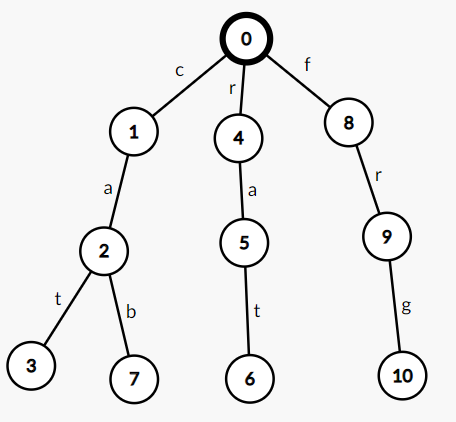
\includegraphics[width=0.4\textwidth,center]{../photo/trie1.png}\\
\indent建立可持久化Trie:\\
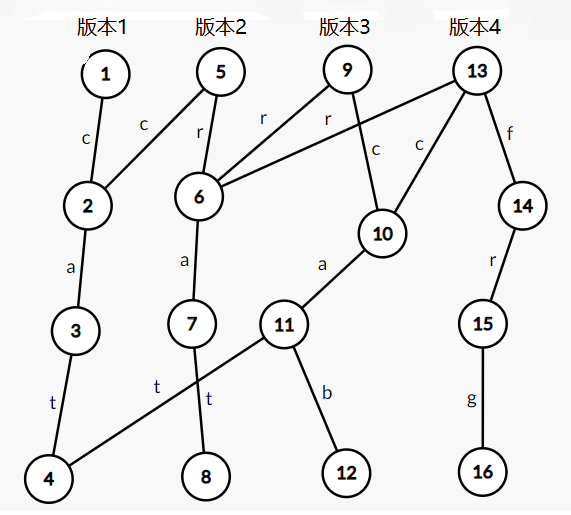
\includegraphics[width=0.4\textwidth,center]{../photo/trie2.png}\\
\begin{lstlisting}[language=c++,escapeinside=``]
void insert(int q,int p,int x)//`将x插入版本p的根中,版本p的上一个版本为版本q`
{
    max_id[q]=x; //`max\_id纪录了该位置下可以找到的最新版本编号`
    for(int i=24;i>=0;i--)
    {
        int u=(sum[x]>>i)&1;
        if(q) trie[p][!u]=trie[q][!u];
        trie[p][u]=++idx;max_id[idx]=x;
        q=trie[q][u],p=idx;
    }
}
void query(int l,int r,int x)//`查询第l个到第r个数字中异或x得到的最大值`
{
    int p=root[r],ans=0;
    for(int i=24;i>=0;i--)
    {
        int u=(x>>i)&1;
        if(trie[p][!u] && max_id[trie[p][!u]]>=l)
        {
            ans+=(1<<i);p=trie[p][!u];
        }
        else p=trie[p][u];
    }
    printf("%d\n",ans);
}
\end{lstlisting}
\section{KMP}
\begin{lstlisting}[language=c++,escapeinside=``]
void getnext(char S[])
{
    int l=strlen(S+1);
    Next[1]=0;
    for(int i=2,k=0;i<=l;i++)
    {
        while(k && S[i]!=S[k+1]) k=Next[k];
        if(S[i]==S[k+1]) k++;
        Next[i]=k;
    }
}
int kmp(char P[],char S[])
{
    int lp=strlen(P+1),ls=strlen(S+1);
    for(int i=1,j=1;i<=lp;i++) //`i为主串指针,j为模式串指针`
    {
        while(j>1 && P[i]!=S[j]) j=Next[j-1]+1;
        if(P[i]==S[j]) j++;
        if(j==ls+1) return i-ls+1;
    }
    return -1;
}
\end{lstlisting}
\subsubsection{Border树}
\indent1.每个前缀Prefix[i]的所有Border:节点i到根的链。\\
\indent2.哪些前缀有长度为$x$的Border:$x$的子树。\\
\indent3.求两个前缀的公共Border等价于求LCA。\\
\subsubsection{字符串的周期}
\indent p是S的周期=$|$S$|-$p是S的Border,S的Border的Border也是S的Border。\\
\subsubsection{统计每个前缀的出现次数}
\indent统计每个前缀Prefix[i]在同一个字符串的出现次数。
\begin{lstlisting}[language=c++,escapeinside=``]
for(int i=1;i<=n;i++) ans[nex[i]]++;
for(int i=n;i>=1;i--) ans[nex[i]]+=ans[i];
for(int i=1;i<=n;i++) ans[i]++;
\end{lstlisting}
\indent考虑第二个问题,字符串S的每个前缀在字符串T中的出现次数是多少。构造字符串S+\#+T,对新字符串长度$\ge n$的部分进行上面的操作即可。\\
\section{拓展KMP}
\begin{lstlisting}[language=c++,escapeinside=``]
// `exkmp(s,n,s,n,nxt,nxt) 求字符串s的Zbox`
// `exkmp(t,m,s,n,ext,nxt) 求字符串t的后缀与s的LCP`
void exkmp(char *s,int lens,char *t,int lent,int *ext,int *nxt)
{
    ext[0]=0;
    for(int i=1,l=0,r=0;i<=lens;i++)
    {
        ext[i]=i<=r?min(nxt[i-l+1],r-i+1):0;
        while(i+ext[i]<=lens && ext[i]<lent && s[i+ext[i]]==t[ext[i]+1]) ext[i]++;
        if(i+ext[i]-1>=r && i!=1) l=i,r=i+ext[i]-1;
    }
}
\end{lstlisting}
\section{AC自动机}
\indent KMP:一个模式串在一个主串上匹配。AC自动机:多个模式串在主串上匹配。\\
\indent1.Trie树构建的复杂度是$O(m\times len)$,其中$m$为模式串数量,$len$为模式串平均长度。\\
\indent2.构建fail指针时,时间也是线性的。\\
\indent3.在匹配时,最耗时的是fail指针的跳动,每次最多前跳$len$次,若主串长度为$n$,那么总匹配时间复杂度为$O(n*len)$。
\begin{lstlisting}[language=c++,escapeinside=``]
void insert(char s[])
{
    int p=0,l=strlen(s);
    for(int i=0;i<l;i++)
    {
        int u=s[i]-'a';
        if(!trie[p][u]) trie[p][u]=++cnt;
        p=trie[p][u];		
    }
    son[p]++;
}
void make_fail()
{
    queue<int>q;
    for(int i=0;i<26;i++)
        if(trie[0][i]) q.push(trie[0][i]);
    while(!q.empty())
    {
        int t=q.front(); q.pop();
        for(int i=0;i<26;i++)
        {
            int p=trie[t][i];
            if(!p) trie[t][i]=trie[fail[t]][i];
            else
            {
                fail[p]=trie[fail[t]][i];
                q.push(p);
            }
        }
    }
}
int query(char s[]) //`查询多少模式串在字符串s中出现过`
{
    int nn=0;
    int num=0,l=strlen(s);
    for(int i=0,j=0;i<l;i++)
    {
        int t=s[i]-'a';j=trie[j][t];
        int p=j;
        while(p && ~son[p])
        {
            nn++;num+=son[p];
            son[p]=-1;p=fail[p];
        }
    }
    return num;
}
\end{lstlisting}
\subsubsection{AC自动机上拓扑排序}
假设当前的位置为$p$,这意味着我们当前匹配到了$p$以及$p$的fail链上的所有位置。所以对fail树进行拓扑排序可较快求解。
\begin{lstlisting}[language=c++]
for(int i=1;i<=cnt;i++) d[fail[i]]++;
for(int i=1;i<=cnt;i++) if(d[i]==0) q.push(i);
while(!q.empty())
{
    int u=q.front();q.pop();
    d[fail[u]]--;ans[fail[u]]+=ans[u];
    if(d[fail[u]]==0) q.push(fail[u]);
}
\end{lstlisting}
\subsubsection{last指针优化}
在自动机上跳fail时,有时不得不遍历一些无用的fail结点,我们将fail链压缩,压缩为只包含关键结点的last指针。时间复杂度为$O(\sqrt n)$。
\subsubsection{AC自动机结合DP}
通常先对son数组进行预处理,常见的有在BFS过程中:son[t]$\mid=$son[fail[t]]或son[t]$+=$son[fail[t]]。
\begin{lstlisting}[language=c++]
for(int i=1;i<=len;i++)
{
    for(int j=0;j<=cnt;j++)
    {
        for(int u=0;u<26;u++)
        {
            f[i][trie[j][u]]=max(f[i][trie[j][u]],f[i-1][j]+son[trie[j][u]]);
            ans=max(ans,f[i][trie[j][u]]);
        }
    }
}
\end{lstlisting}
\subsubsection{fail树上DFS序+数据结构操作}
\indent由于AC自动机属于离线算法,有时候我们会遇到一些需要在线维护更新的题目。将AC自动机上的fail指针全部反过来,就得到了fail树。这种题目一般是利用fail树上的性质,配合数据结构(差分,树状数组,离线,树剖)来变成树论中的数据结构问题。\\
\indent遇到这种问题,首先要想清楚如何在fail树上处理单组询问,不断尝试用数据结构优化即可。\\
\noindent常见数据结构技巧:\\
\indent1.询问某结点子树下的数字之和。使用DFS序将结点映射为序列,$u$结点代表的子树序列为$L[u],R[u]$(入栈时间和出栈时间)。\\
\indent2.将某结点子树下的权值统一加一。可使用上述DFS序用树状数组区间修改。或者使用树状数组维护一个差分数组,$u$结点子树都加一,等于$L[x]$加$1$,$R[x]+1$减$1$。\\
\indent3.将链上的值统一加一。使用树剖。或者用树状数组维护树上差分,差分后某点/边的值等于子树之和,用1求解。
\section{Manacher}
\begin{lstlisting}[language=c++]
int manacher(char S[],int P[],char New[])
{
    int len=0,k=1,l=strlen(S+1);
    New[k]='#';
    for(int i=1;i<=l;i++)
    {
        New[++k]=S[i];New[++k]='#';
    }
    int mx=0,mid;
    for(int i=1;i<=k;i++)
    {
        if(i<mx) P[i]=min(mx-i,P[2*mid-i]);
        else P[i]=1;
        while(i-P[i]>=1 && i+P[i]<=k && New[i-P[i]]==New[i+P[i]]) P[i]++;
        if(i+P[i]>mx)
        {
            mx=i+P[i];mid=i;len=max(len,P[i]);
        }
    }
    return len-1; //找到的最长回文长度
}
\end{lstlisting}
\section{回文自动机}
\indent对于一个字符串$s$,它的本质不同回文子串个数最多只有$|s|$个。因此回文树状态数是$|s|$的。对于每一个状态,它实际只代表一个本质不同的回文子串,即转移到该节点的状态唯一,因此总转移数也是$|s|$的。\\
\indent和其它的自动机一样,一个节点的fail指针指向的是这个节点所代表的\textbf{回文串的最长回文后缀}所对应的节点,但是转移边并非代表在原节点代表的回文串后加一个字符,而是表示在原节点代表的回文串前后各加一个相同的字符。\\
\indent回文树有两个初始状态,分别代表长度为$-1,0$的回文串。我们可以称它们为奇根,偶根。它们不表示任何实际的字符串,仅作为初始状态存在。考虑构造完前$p-1$个字符的回文树后,向自动机中添加在原串里位置为$p$的字符。我们从以上一个字符结尾的最长回文子串对应的节点开始,不断沿着fail指针走,直到找到一个节点p满足s[i]=s[i-len[p]-1],即满足此节点所对应回文子串的上一个字符与待添加字符相同。构造时间复杂度$O(|s|)$\\
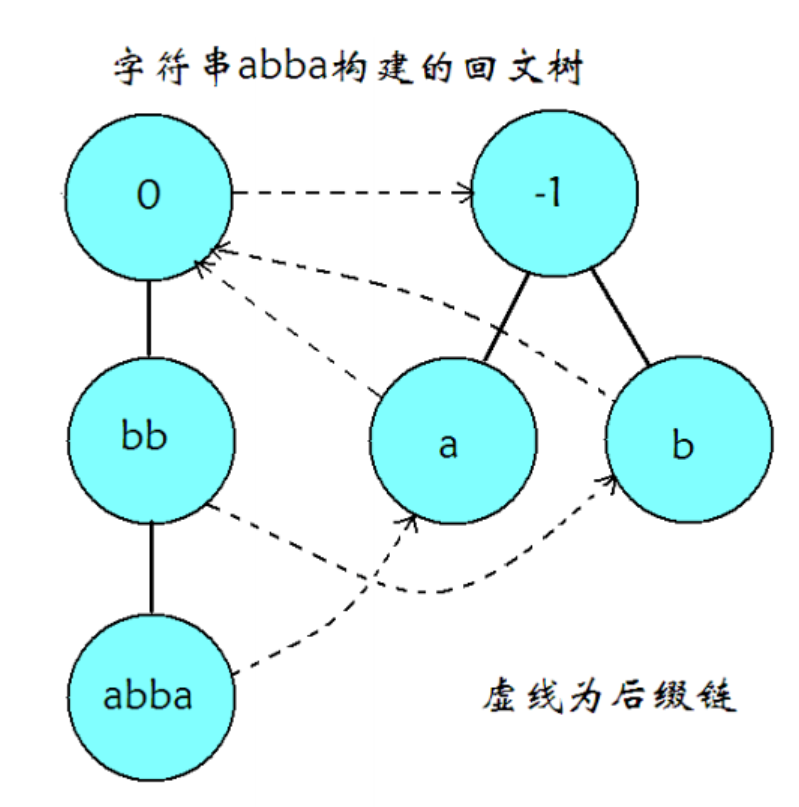
\includegraphics[width=0.4\textwidth,center]{../photo/pam}\\
\begin{lstlisting}[language=c++,escapeinside=``]
struct PAM
{
    int len[maxn],ch[maxn][26],fail[maxn],cnt;
    char s[maxn];
    PAM()
    {
        len[1]=-1;len[0]=0;fail[1]=0;fail[0]=1;cnt=1;
    }
    int get_fail(int x,int i) //`看看x的fail链上哪个可以接上s[i]`
    {
        while(s[i-len[x]-1]!=s[i]) x=fail[x];
        return x;
    }
    void insert()
    {
        int l=strlen(s+1),p=0;
        for(int i=1;i<=l;i++)
        {
            int u=s[i]-'a',pos=get_fail(p,i);
            if(!ch[pos][u])
            {
                fail[++cnt]=ch[get_fail(fail[pos],i)][u];
                ch[pos][u]=cnt;len[cnt]=len[pos]+2;
            }
            p=ch[pos][s[i]-'a'];
        }
    }
}pam;
\end{lstlisting}
\subsubsection{本质不同回文子串个数}
一个串的本质不同回文子串个数等于回文树的状态数(排除奇根和偶根两个状态)。
\subsubsection{回文子串出现次数}
建出回文树,使用类似后缀自动机统计出现次数的方法。由于回文树的构造过程中,节点本身就是按照拓扑序插入,因此只需要逆序枚举所有状态,将当前状态的出现次数加到其fail指针对应状态的出现次数上即可。
\begin{lstlisting}[language=c++]
void build()
{
    for(int i=cnt;i>=0;i--) sz[fail[i]]+=sz[i];
}
\end{lstlisting}
也可以在字符插入的过程维护nump[u]=nump[fail[u]]+1,即求出字符串当前位置结尾的字符串数量,统计插入过程的所有nump[u]之和即可。
\subsubsection{双向插入PAM}
由于回文串的特殊性,PAM在建造时可以从字符串一个位置出发,向左右两边用时插入字符,这需要维护两个结束结点pre和last,当插入字符后发现整个字符串就是一个回文串时,要同时更新pre和last。
\begin{lstlisting}[language=c++]
void insert_front(int x,int c)
{
    while(s[x]!=s[x+len[pre]+1]) pre=fail[pre];
    if (!ch[pre][c]) 
    {
        len[++cnt]=len[pre]+2;
        int j=fail[pre];while(s[x+len[j]+1]!=s[x]) j=fail[j];
        fail[cnt]=ch[j][c];ch[pre][c]=cnt;
        nump[cnt]=nump[fail[cnt]]+1;
    }
    pre=ch[pre][c];
    if(len[pre]==r-l+1) last=pre; //若本身为回文串更新last
    sum=sum+nump[pre]; //所有回文串总数
}
void insert_back(int x,int c)
{
    while(s[x]!=s[x-len[last]-1]) last=fail[last];
    if (!ch[last][c]) 
    {
        len[++cnt]=len[last]+2;
        int j=fail[last];while(s[x-len[j]-1]!=s[x]) j=fail[j];
        fail[cnt]=ch[j][c];ch[last][c]=cnt;
        nump[cnt]=nump[fail[cnt]]+1;
    }
    last=ch[last][c];
    if(len[last]==r-l+1) pre=last; //若本身为回文串更新pre
    sum=sum+nump[last]; //所有回文串总数
}
\end{lstlisting}

\section{后缀数组}
\indent将字符串的所有后缀进行字典序排序,令$sa[i]$代表排名第$i$的后缀字符串的起始位置的下标,$rk[i]$代表从第$i$位开始的后缀字符串的排名,这两个数组满足性质:$sa[rk[i]]=rk[sa[i]]=i$。\\
\subsection{倍增}
\indent使用倍增的思想,先对每个长度为$1$的子串(即每个字符)进行排序。\\
\indent$S[i,k]$表示从$i$开始,长度为$2^k$的字符串,则$S[i,k+1]=S[i,k]+S[i+2^k,k]$。\\
\indent用上一轮排好的顺序,两两组合,进行双关键字排序($pair$排序),即可用长度为$k$的排名推出长度为$k+1$的排名。\\
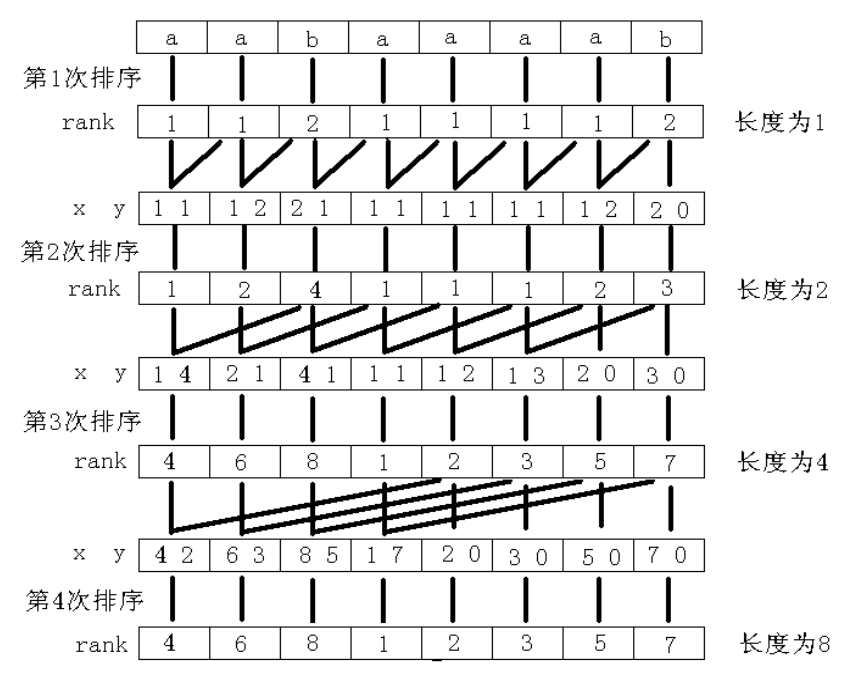
\includegraphics[width=0.7\textwidth,center]{../photo/sa2}\\
\indent如果使用$sort$进行排序,共需排序$\log n$次,时间复杂度$O(n\log ^2n)$,使用基数排序将排序时间优化至$O(n)$,于是总体时间复杂度被优化到了$O(n\log n)$。
\begin{lstlisting}[language=c++,escapeinside=``]
struct Suffix_Array
{
    char s[maxn];
    int n,m=122,x[maxn],y[maxn];
    int rk[maxn],sa[maxn],height[maxn],c[maxn];
    void get_SA() //`记得对n初始化`
    {
        memset(height,0,sizeof(height));
        memset(rk,0,sizeof(rk));
        memset(y,0,sizeof(y));
        for(int i=1;i<=m;i++) c[i]=0;
        for(int i=1;i<=n;i++) c[x[i]=s[i]]++;
        for(int i=1;i<=m;i++) c[i]+=c[i-1];
        for(int i=n;i>=1;i--) sa[c[x[i]]--]=i; //`基数排序先计算出长度为1子串的顺序`
        for(int k=1;k<=n;k<<=1)
        {
            int num=0;
            //`y[i]表示第二关键字排名为i的数,第一关键字的位置`
            //`第n-k+1到第n位是没有第二关键字的,所以排名在最前面`
            for(int i=n-k+1;i<=n;i++) y[++num]=i; 
            for(int i=1;i<=n;i++) if(sa[i]>k) y[++num]=sa[i]-k;
            for(int i=1;i<=m;i++) c[i]=0;
            for(int i=1;i<=n;i++) c[x[i]]++;
            for(int i=1;i<=m;i++) c[i]+=c[i-1];
            //`因为y的顺序是按照第二关键字的顺序来排的`
            //`第二关键字靠后的,在同一个第一关键字桶中排名越靠后`
            for(int i=n;i>=1;i--) sa[c[x[y[i]]]--]=y[i],y[i]=0;
            for(int i=1;i<=n;i++) swap(x[i],y[i]);
            x[sa[1]]=1;num=1; 
            //合并并列排名
            for(int i=2;i<=n;i++) 
           x[sa[i]]=(y[sa[i]]==y[sa[i-1]]&&y[sa[i]+k]==y[sa[i-1]+k])?num:++num;
            if(num==n) break; m=num;
        }
        int k=0;height[1]=0;
        for(int i=1;i<=n;i++) rk[sa[i]]=i;
        for(int i=1;i<=n;i++)
        {	
            if(rk[i]==1) continue;
            if(k) k--;
            int j=sa[rk[i]-1];
            while(i+k<=n&&j+k<=n&&s[i+k]==s[j+k]) k++;
            height[rk[i]]=k;
        }
    }
}s1,s2;
\end{lstlisting}
\subsection{SA-IS}
\begin{lstlisting}[language=c++,escapeinside=``]
struct SAIS
{
    int sa[maxn],rk[maxn],s[maxn*2],op[maxn*2],pos[maxn*2];
    int c1[maxn],c[maxn],ht[maxn];
    char str[maxn];
    #define L(x) sa[c[s[x]]--]=x
    #define R(x) sa[c[s[x]]++]=x
    inline void sa_sort(int *S,int n,int m,int *s,int *op,int tn)
    {
        for(int i=1;i<=n;i++) sa[i]=0;
        for(int i=1;i<=m;i++) c1[i]=0;
        for(int i=1;i<=n;i++) c1[s[i]]++;
        for(int i=2;i<=m;i++) c1[i]+=c1[i-1];
        for(int i=1;i<=m;i++) c[i]=c1[i];
        for(int i=tn;i;i--) L(S[i]);
        for(int i=1;i<=m+1;i++) c[i]=c1[i-1]+1;
        for(int i=1;i<=n;i++)
        if(sa[i]>1 && op[sa[i]-1]) R(sa[i]-1);
        for(int i=1;i<=m;i++) c[i]=c1[i];
        for(int i=n;i;i--)
        if(sa[i]>1 && !op[sa[i]-1]) L(sa[i]-1);
    }
    void SA_IS(int n,int m,int *s,int *op,int *pos)//`m代表字符的范围`
    {
        int tot=0,cnt=0;int *S=s+n;
        op[n]=0;
        for(int i=n-1;i;i--) op[i]=(s[i]!=s[i+1])?s[i]>s[i+1]:op[i+1];
        rk[1]=0;
        for(int i=2;i<=n;i++)
        if(op[i-1]==1 && op[i]==0) pos[++tot]=i,rk[i]=tot;
        else rk[i]=0;
        sa_sort(pos,n,m,s,op,tot);
        int u=0,p=0;
        for(int i=1;i<=n;i++)
        if(rk[sa[i]])
        {
            u=rk[sa[i]];
            if(cnt<=1 || pos[u+1]-pos[u]!=pos[p+1]-pos[p]) ++cnt;
            else
            {
                for(int j=0;j<=pos[u+1]-pos[u];j++)
                if(s[pos[u]+j]!=s[pos[p]+j]||op[pos[u]+j]!=op[pos[p]+j])
                {++cnt;break;}
            }
            S[u]=cnt;
            p=u;
        }
        if(tot!=cnt) SA_IS(tot,cnt,S,op+n,pos+n);
        else for(int i=1;i<=tot;i++) sa[S[i]]=i;
        for(int i=1;i<=tot;i++) S[i]=pos[sa[i]];
        sa_sort(S,n,m,s,op,tot);
    }
    void get_ht(int n) //ht[1]=1
    {
        for(int i=1;i<=n;i++) rk[sa[i]=sa[i+1]]=i;
        for(int i=1,p=0;i<=n;ht[rk[i]]=p,i++)
        if(rk[i]!=1) 
        for(p=p-!!p;sa[rk[i]-1]+p<=n && i+p<=n&&s[i+p]==s[sa[rk[i]-1]+p];p++);
    }
    void Get_SA(int n)
    {
        for(int i=1;i<=n;i++) s[i]=str[i];
        s[++n]=1;SA_IS(n--,122,s,op,pos);//`122为字符串的ASCII码范围`
        get_ht(n);
    }
}sa;
\end{lstlisting}
\subsubsection{寻找最小的循环移动位置}
将字符串$S$复制一份变成$SS$就转化成了后缀排序问题。
\subsubsection{从字符串首尾取字符最小化字典序}
需要在原串后缀与反串后缀构成的集合内比较大小,可以将反串拼接在原串后,并在中间加上一个没出现过的字符(如\#,代码中可以直接使用空字符),求后缀数组,即可$O(1)$完成这一判断。
\subsubsection{LCP(最长公共前缀)}
\indent定义$LCP(i,j)$为$suff(i)$和$suff(j)$的最长公共前缀。那么$height[i]=LCP(sa[i],sa[i-1])$,即第$i$名的后缀与它前一名的后缀的最长公共前缀,$height[1]=0$。\\
\indent$height[rk[i]]\ge height[rk[i-1]]-1$。
\subsubsection{两子串最长公共前缀}
$LCP(sa[i],sa[j])=\min\{height[i+1..j]\}$,于是就转换为了RMQ问题。
\begin{lstlisting}[language=c++]
void get_ST()
{
    for(int i=1;i<=n;i++) st[i][0]=height[i];
    for(int j=1;j<16;j++)
    {
        for(int i=1;i+(1<<(j-1))<=n;i++)
        {
            st[i][j]=min(st[i][j-1],st[i+(1<<(j-1))][j-1]);
        }
    }
}
int LCP(int l,int r)
{
    l=rk[l],r=rk[r];
    if(l>r) swap(l,r); l++;
    int k=log2(r-l+1);
    return min(st[l][k],st[r-(1<<k)+1][k]);
}
\end{lstlisting}
\subsubsection{比较一个字符串的两个子串的大小关系}
\indent假设需要比较的是$A[a..b]$和$B[c..d]$的大小关系。\\
\indent若$LCP(a,c)\ge \min(|A,|B|)$,$A<B \iff |A|<|B|$。否则,$A<B \iff rk[a]<rk[c]$。
\subsubsection{不同子串的数目}
\indent子串就是后缀的前缀,所以可以枚举每个后缀,计算前缀总数,再减掉重复。“前缀总数”其实就是子串个数,为$n(n+1)/2$。\\
\indent如果按后缀排序的顺序枚举后缀,每次新增的子串就是除了与上一个后缀的LCP剩下的前缀。这些前缀一定是新增的,否则会破坏$LCP(sa[i],sa[j])$的性质。只有这些前缀是新增的,因为LCP部分在枚举上一个前缀时计算过了。\\
\indent所以答案为$n(n+1)/2-\displaystyle\sum_{i=2}^{n}height[i]$。
\subsubsection{连续的若干个相同子串}
我们可以枚举连续串的长度$|S|$,按照$|S|$对整个串进行分块,对相邻两块的块首进行LCP与LCS查询。\\
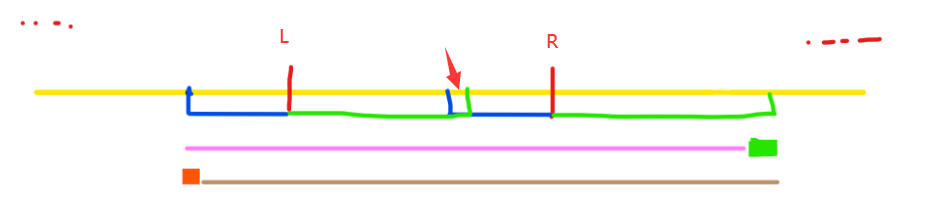
\includegraphics[width=0.7\textwidth,center]{../photo/sa3}\\
\begin{lstlisting}[language=c++,title=字符串多少子串可写成AABB形式]
for(int len=1;len<=n/2;len++)
{
    for(int i=1;i<=n;i+=len)
    {
        int l=i,r=i+len;int lcp=s1.LCP(l,r);lcp=min(lcp,len);
        int L=n-r+2,R=n-l+2;int lcs=s2.LCP(L,R);lcs=min(lcs,len-1);
        if(lcs+lcp>=len)
        {
            int t=lcs+lcp-len;
            b[i-lcs]++;b[i-lcs+t+1]--;
            a[r+lcp-1-t]++;a[r+lcp]--;
        }
    }
}
for(int i=1;i<=n;i++) a[i]+=a[i-1],b[i]+=b[i-1];
ll ans=0; for(int i=1;i<n;i++) ans+=a[i]*b[i+1];
\end{lstlisting}
\subsubsection{结合并查集}
某些题目求解时要求你将后缀数组划分成若干个连续LCP长度大于等于某一值的段,亦即将$h$数组划分成若干个连续最小值大于等于某一值的段并统计每一段的答案。如果有多次询问,我们可以将询问离线。观察到当给定值单调递减的时候,满足条件的区间个数总是越来越少,而新区间都是两个或多个原区间相连所得,且新区间中不包含在原区间内的部分的$h$值都为减少到的这个值。我们只需要维护一个并查集,每次合并相邻的两个区间,并维护统计信息即可。
\subsubsection{结合单调栈}
有些时候我们需要计算$\sum LCP$,使用单调栈,找到每个$height$向左向右可以覆盖的有效范围,直接计算即可。
\begin{lstlisting}[language=c++]
vector<int>st;
for(int i=2;i<=SA.n;i++)
{
    while(!st.empty() && SA.height[st.back()]>SA.height[i]) st.pop_back();
    if(st.empty()) l[i]=1;
    else l[i]=st.back();
    st.pb(i);
}
st.clear();
for(int i=SA.n;i>=2;i--)
{
    while(!st.empty() && SA.height[st.back()]>=SA.height[i]) st.pop_back();
    if(st.empty()) r[i]=SA.n+1;
    else r[i]=st.back();
    st.pb(i);
}
for(int i=2;i<=SA.n;i++) ans+=(r[i]-i)*(i-l[i])*SA.height[i];
\end{lstlisting}
\section{后缀自动机}
在SAM中状态数最多有$2*n-1$个,转移数最多$3n-4$。
\begin{itemize}
    \item $s$的子串可以根据它们结束的位置$\operatorname{endpos}$被划分为多个等价类。
    \item SAM由初始状态$t_0$和与每一个$\operatorname{endpos}$等价类对应的每个状态组成。
    \item 对于每一个状态$v$,一个或多个子串与之匹配。我们记$\operatorname{longest}(v)$为其中最长的一个字符串,记$\operatorname{len}(v)$为它的长度。类似地,记$\operatorname{shortest}(v)$为最短的子串,它的长度为$\operatorname{minlen}(v)$。那么对应这个状态的所有字符串都是字符串$\operatorname{longest}(v)$的不同的后缀,且所有字符串的长度恰好覆盖区间$[\operatorname{minlen}(v),\operatorname{len}(v)]$中的每一个整数。
    \item 对于任意不是$t_0$的状态$v$,定义后缀链接为连接到对应字符串$\operatorname{longest}(v)$的长度为$\operatorname{minlen}(v)-1$的后缀的一条边。从根节点$t_0$出发的后缀链接可以形成一棵树。这棵树也表示$\operatorname{endpos}$集合间的包含关系。
    \item 对于$t_0$以外的状态$v$,可用后缀链接$\operatorname{link}(v)$表达$\operatorname{minlen}(v)$:$\operatorname{minlen}(v)=\operatorname{len}(\operatorname{link}(v))+1$。
    \item 如果我们从任意状态$v_0$开始顺着后缀链接遍历,总会到达初始状态$t_0$。这种情况下我们可以得到一个互不相交的区间$[\operatorname{minlen}(v_i),\operatorname{len}(v_i)]$的序列,且它们的并集形成了连续的区间$[0,\operatorname{len}(v_0)]$。
\end{itemize}
\begin{lstlisting}[language=c++]
struct SAM
{
    int idx,last,len[maxn*2],link[maxn*2],nex[maxn*2][26],sz[maxn*2];
    SAM()
    {
        idx=0;last=0;len[0]=0;link[0]=-1;
    }
    void insert(int c)
    {
        int cur=++idx;
        len[cur]=len[last]+1;sz[cur]=1;
        int p=last;
        while(p!=-1 && !nex[p][c]) nex[p][c]=cur,p=link[p];
        if(p==-1) link[cur]=0;
        else
        {
            int q=nex[p][c];
            if(len[p]+1==len[q]) link[cur]=q;
            else
            {
                int clone=++idx;
                len[clone]=len[p]+1;link[clone]=link[q];sz[clone]=0;
                for(int i=0;i<26;i++) nex[clone][i]=nex[q][i];
                while(p!=-1 && nex[p][c]==q) nex[p][c]=clone,p=link[p];
                link[q]=link[cur]=clone;
            }
        }
        last=cur;
    }
}sam;
\end{lstlisting}
\subsubsection{结点代表的子串出现的次数即字符串上的结尾位置}
\begin{lstlisting}[language=c++]
int c[2*maxn],a[2*maxn];
void build(int n)
{
    int now=1;
    for(int i=1;i<=n;i++) endpos[now=nex[now][s[i]-'a']]=i;
    for(int i=1;i<=idx;i++) c[len[i]]++;
    for(int i=1;i<=n;i++) c[i]+=c[i-1];
    for(int i=idx;i>=1;i--) a[c[len[i]]--]=i;
    for(int i=idx;i>=1;i--) 
    {
        int pos=a[i];sz[link[pos]]+=sz[pos];
        if(!endpos[link[pos]]) endpos[link[pos]]=endpos[pos];
    }
}
\end{lstlisting}
\subsubsection{不同子串个数}
每个节点对应的子串数量是$\operatorname{len}(i)-\operatorname{len}(\operatorname{link}(i))$,对自动机所有节点求和即可。
\subsubsection{所有不同子串的总长度}
每个节点对应的所有后缀长度是$\frac{\operatorname{len}(i)\times(\operatorname{len}(i)+1)}{2}$,减去其$\operatorname{link}$节点的对应值就是该节点的净贡献,对自动机所有节点求和即可。
\subsubsection{字典序第$k$大子串}
字典序第$k$大的子串对应于SAM中字典序第$k$大的路径,因此在计算每个状态的路径数后,我们可以很容易地从SAM的根开始找到第$k$大的路径。预处理的时间复杂度为$O(|S)$,单次查询的复杂度为$O(|ans|\cdot|\Sigma|)$(其中$|ans|$是查询的答案,$|\Sigma|$为字符集的大小)。
\begin{lstlisting}[language=c++,escapeinside=``]
void dfs(int pos,int num)
{
    if(num<=sz[pos]) return;
    num-=sz[pos];
    for(int i=0;i<26;i++)
    {
        int p=nex[pos][i];
        if(!p) continue;
        if(sum[p]<num) num-=sum[p];
        else 
        {
            printf("%c",'a'+i);
            dfs(p,num);return;
        }
    }
}
void build(int n)
{
    for(int i=1;i<=idx;i++) c[len[i]]++;
    for(int i=1;i<=n;i++) c[i]+=c[i-1];
    for(int i=idx;i>=1;i--) a[c[len[i]]--]=i;
    for(int i=idx;i>=1;i--) 
    {
        int pos=a[i];sz[link[pos]]+=sz[pos];
        if(t==0) sz[link[pos]]=1;//`t为0则表示不同位置的相同子串算作一个`
    }
    sz[0]=0;
    for(int i=0;i<=idx;i++) sum[i]=sz[i];
    for(int i=idx;i>=0;i--)
    {
        for(int j=0;j<26;j++)
        {
            int pos=nex[a[i]][j];
            if(!pos) continue;
            sum[a[i]]+=sum[pos];
        }
    }
    if(sum[0]<k){puts("-1");return;}
    dfs(0,k);
}
\end{lstlisting}
\subsubsection{最小循环移位}
容易发现字符串$S+S$包含字符串$S$的所有循环移位作为子串。贪心地访问最小的字符即可。总的时间复杂度为$O(|S|)$。
\subsubsection{两个字符串的最长公共子串}
以其中一个字符串建立SAM,另一个串在SAM上转移。
\begin{lstlisting}
void solve()
{
    scanf("%s",s+1);
    int n=strlen(s+1),p=0,l=0,ans=0;
    for(int i=1;i<=n;i++)
    {
        while(p&&!nex[p][s[i]-'a']) p=link[p],l=len[p];
        if(nex[p][s[i]-'a']) p=nex[p][s[i]-'a'],l++,ans=max(ans,l);
    }
    printf("%d\n",ans);
}
\end{lstlisting}
\subsubsection{多个字符串间的最长公共子串}
以其中一个字符串建立SAM,其余串在SAM上转移。
\begin{lstlisting}[language=c++]
void build()
{
    for(int i=1;i<=idx;i++) c[len[i]]++;
    for(int i=1;i<=idx;i++) c[i]+=c[i-1];
    for(int i=idx;i>=1;i--) a[c[len[i]]--]=i;
}
void solve()
{
    memset(mn,0x3f,sizeof(mn));build();
    while(scanf("%s",s+1)!=EOF)
    {
        int n=strlen(s+1),pos=0,l=0;
        for(int i=1;i<=n;i++)
        {
            while(pos&&!nex[pos][s[i]-'a']) pos=link[pos],l=len[pos];
            if(nex[pos][s[i]-'a']) pos=nex[pos][s[i]-'a'],l++;
            mx[pos]=max(mx[pos],l);
        }
        for(int i=idx;i>=1;i--)
        {
            int now=a[i],fa=link[now];
            mx[fa]=max(mx[fa],min(mx[now],len[fa]));
            mn[now]=min(mn[now],mx[now]);mx[now]=0;
        }
    }
    int ans=0;
    for(int i=1;i<=idx;i++) ans=max(ans,mn[i]);
    printf("%d\n",ans);
}
\end{lstlisting}
\subsubsection{区间本质不同字符串个数}
\begin{lstlisting}[language=c++]
#include<bits/stdc++.h>
using namespace std;
typedef long long ll;
const int maxn = 2e5 + 100;
/* 维护最后出现位置在i(左端点)的本质不同串数量 */
struct SegmentTree_Sum{
    ll Sum[maxn * 8],Lazy[maxn*8];
    void down(int x,int l,int mid,int r){
        Sum[x<<1] += Lazy[x] * (mid - l + 1);
        Sum[x<<1|1] += Lazy[x] * (r - mid);
        Lazy[x<<1] += Lazy[x];
        Lazy[x<<1|1] += Lazy[x];
        Lazy[x] = 0;
    }
    void up(int x){Sum[x] = Sum[x<<1] + Sum[x<<1|1];}
    void update(int x,int l,int r,int L,int R,int val){
        if (l > R or L > r)return;
        if (L <= l and r <= R){
            Sum[x] += 1ll * val * (r - l + 1);
            Lazy[x] += val;
            return;
        }
        int mid = l + r >> 1;down(x,l,mid,r);
        update(x<<1,l,mid,L,R,val);update(x<<1|1,mid+1,r,L,R,val);
        up(x);
    }
    ll query(int x,int l,int r,int L,int R){
        if (l > R or L > r)return 0;
        if (L <= l and r <= R)return Sum[x];
        int mid = l + r >> 1;down(x,l,mid,r);
        return query(x<<1,l,mid,L,R) + query(x<<1|1,mid+1,r,L,R);
    }
}segtree;
struct SegmentTree_Max{
    int Max[maxn*8];
    void update(int x,int l,int r,int pos,int val){
        Max[x] = max(Max[x],val);
        if (l == r)return;
        int mid = l + r >> 1;
        if (pos <= mid)update(x<<1,l,mid,pos,val);
        else update(x<<1|1,mid+1,r,pos,val);
    }
    int query(int x,int l,int r,int L,int R){
        if (l > R or L > r)return -1;
        if (L <= l and r <= R)return Max[x];
        int mid = l + r >> 1;
        return max(query(x<<1,l,mid,L,R),query(x<<1|1,mid+1,r,L,R));
    }
}dfstree;
int n,q;
char s[maxn];
ll ans[maxn];
typedef pair<pair<int,int>,int> Query;
vector<Query> query;
struct Suffix_Automaton{
    int nxt[maxn*2][26],fa[maxn*2],l[maxn*2];
    int last,cnt;
    /* 每个color最上边一个点 */
    int up_to[maxn];
    /* 是否被染过色 */
    bool used[maxn*2];
    Suffix_Automaton(){ clear(); }
    void clear(){
        last =cnt=1;fa[1]=l[1]=0;
        memset(nxt[1],0,sizeof nxt[1]);
    }
    void init(char *s){
        while (*s){add(*s-'a');s++;}
    }
    void add(int c){
        int p = last;
        int np = ++cnt;
        memset(nxt[cnt],0,sizeof nxt[cnt]);
        l[np] = l[p]+1;last = np;
        while (p&&!nxt[p][c])nxt[p][c] = np,p = fa[p];
        if (!p)fa[np]=1;
        else{
            int q = nxt[p][c];
            if (l[q]==l[p]+1)fa[np] =q;
            else{
                int nq = ++ cnt;
                l[nq] = l[p]+1;
                memcpy(nxt[nq],nxt[q],sizeof (nxt[q]));
                fa[nq] =fa[q];fa[np] = fa[q] =nq;
                while (nxt[p][c]==q)nxt[p][c] =nq,p = fa[p];
            }
        }
    }
    vector<int> E[maxn * 2];
    int in[maxn*2],out[maxn*2],dfn;
    void dfs(int u){
        in[u] = ++dfn;
        for (int v:E[u])dfs(v);
        out[u] = dfn;
    }
    void gao(){
        for (int i=2;i<=cnt;i++)E[fa[i]].push_back(i);
        dfs(1);
        for (int i=1,now = 1;i<=n;i++){
            now = nxt[now][s[i] - 'a'];
            assert(l[now] == i);
            segtree.update(1,1,n,1,i,1);
            int u = now;
            while (u != 1 and !used[u]){
                used[u] = true;
                u = fa[u];
            }
            while (u != 1){
                int cur = dfstree.query(1,1,cnt,in[u],out[u]);
                segtree.update(1,1,n,cur - l[u]+1,cur - l[up_to[cur]],-1);
                swap(up_to[cur],u);
            }
            dfstree.update(1,1,cnt,in[now],i);
            up_to[i] = 1;
            while (!query.empty() and query.back().first.second == i){
                int l = query.back().first.first;
                int id = query.back().second;
                ans[id] = segtree.query(1,1,n,l,i);
                query.pop_back();
            }
        }
    }
}sam;
int main(){
    scanf("%s%d",s+1,&q);n=strlen(s+1);
    sam.init(s+1);
    for(int i=1;i<=q;i++){
        int l,r;scanf("%d%d",&l,&r);
        query.push_back({{l,r},i});
    }
    sort(query.begin(),query.end(),[](Query x,Query y){
        return x.first.second > y.first.second;
    });
    sam.gao();
    for(int i=1;i<=q;i++) cout<<ans[i]<<endl;
}
\end{lstlisting}
\section{广义后缀自动机}
后缀自动机是用于处理单个字符串的子串问题的强力工具。而广义后缀自动机则是将后缀自动机整合到字典树中来解决对于多个字符串的子串问题。
\subsection{伪广义后缀自动机}
\begin{enumerate}
    \item 通过用特殊符号将多个串直接连接后,再建立SAM。
    \item 对每个串,重复在同一个SAM上进行建立,每次建立前,将last指针置零。
\end{enumerate}
实现方式简单,而且在面对题目时通常可以达到和广义后缀自动机一样的正确性。但是时间复杂度较为危险。
\subsection{构造广义后缀自动机}
\begin{enumerate}
    \item 将所有字符串插入到字典树中。
    \item 从字典树的根节点开始进行BFS,记录下顺序以及每个节点的父亲节点。
    \item 将得到的BFS序列按照顺序,对每个节点在原字典树上进行构建,注意不能将len小于当前len的数据进行操作。
\end{enumerate}
\indent使用广义后缀自动机解决问题时,建议不要在建立自动机时打标记,最好等自动机建好后遍历字符串打标机,或者直接建立$link$树DFS。
\begin{lstlisting}[language=c++]
struct GSA
{
    int nex[maxn][26],idx,len[maxn*2],link[maxn*2];
    GSA()
    {
        link[0]=-1;
    }
    void insert_trie(char *s)
    {
        int p=0,l=strlen(s+1);
        for(int i=1;i<=l;i++)
        {
            int u=s[i]-'a';
            if(!nex[p][u]) nex[p][u]=++idx;
            p=nex[p][u];
        }
    }
    int insert_sam(int last,int u)
    {
        int cur=nex[last][u];
        if(len[cur]) return cur;
        len[cur]=len[last]+1;
        int p=link[last];
        while(p!=-1 && !nex[p][u]) nex[p][u]=cur,p=link[p];
        if(p==-1) link[cur]=0;
        else 
        {
            int q=nex[p][u];
            if(len[p]+1==len[q]) link[cur]=q;
            else
            {
                int clone=++idx;
                len[clone]=len[p]+1;
                link[clone]=link[q];
                for(int i=0;i<26;i++) 
                    nex[clone][i]=len[nex[q][i]]!=0?nex[q][i]:0;
                while(p!=-1 && nex[p][u]==q) nex[p][u]=clone,p=link[p];
                link[q]=link[cur]=clone;
            }
        }
        return cur;
    }
    void build()
    {
        queue<pair<int,int>>q;
        for(int i=0;i<26;i++) if(nex[0][i]) q.push({0,i});
        while(!q.empty())
        {
            auto item=q.front();q.pop();
            int last=insert_sam(item.first,item.second);
            for(int i=0;i<26;i++) if(nex[last][i]) q.push({last,i});
        }
    }
}sam;
\end{lstlisting}
\section{最小表示法}
\subsubsection{循环同构}
当字符串$S$中可以选定一个位置$i$满足$S[i\cdots n]+S[1\cdots i-1]=T$则称$S$与$T$循环同构。
\subsubsection{最小表示}
字符串$S$的最小表示为与$S$循环同构的所有字符串中字典序最小的字符串。
\subsubsection{算法核心}
考虑对于一对字符串在原字符串$S$中的起始位置分别为$i,j$,且它们的前$k$个字符均相同,即$S[i\cdots i+k-1]=S[j\cdots j+k-1]$。假设$S[i+k]>S[j+j]$,我们发现起始位置下标$l$满足$i\leq l\leq i+k$的字符串均不能成为答案。因为对于任意一个字符串$S_{i+p}$一定存在字符串$S_{j+p}$比它更优。所以我们比较时可以跳过下标$l\in[i,i+k]$, 直接比较$S_{i+k+1}$。时间复杂度$O(n)$。 
\begin{lstlisting}[language=c++]
int minshow()//下标从0开始,方便取模
{
    int k=0,i=0,j=1;
    while(k<n&&i<n&&j<n) 
    {
        if(s[(i+k)%n]==s[(j+k)%n]) k++;
        else 
        {
            s[(i+k)%n]>s[(j+k)%n]?i=i+k+1:j=j+k+1;
            if(i==j) i++; k=0;
        }
    }
    return min(i,j);
}
\end{lstlisting}
\section{Lyndon分解}
\indent对于字符串$S$,如果$S$的字典序严格小于$S$的所有后缀的字典序,我们称$S$为Lyndon串。\\
\indent串$S$的Lyndon分解记为$S=w_1w_2\cdots w_k$,其中所有$w_i$为Lyndon串,并且他们的字典序按照非严格单减排序,即$w_i\ge w_{i+1}$。可以发现,这样的分解存在且唯一。
\subsubsection{Duval算法}
\indent如果一个字符串$t$能够分解为$t=ww\cdots\overline{w}$的形式,其中$w$是一个Lyndon串,而$\overline{w}$是$w$的前缀(可能是空串),那么称$\overline{w}$是近似Lyndon串。一个Lyndon串也是近似Lyndon串。\\
\indent Duval算法运用了贪心的思想。算法过程中我们把串$S$分成三个部分$S=s_1s_2s_3$,其中$s_1$是一个Lyndon串,它的Lyndon分解已经记录;$s_2$是一个近似Lyndon串;$s_3$是未处理的部分。\\
\indent定义一个指针$i$指向$s_2$的首字符,则$i$从$1$遍历到$n$(字符串长度)。在循环的过程中我们定义另一个指针$j$指向$s_3$的首字符,指针$k$指向$s_2$中我们当前考虑的字符(意义是$j$在$s_2$的上一个循环节中对应的字符)。我们的目标是将$s[j]$添加到$s_2$的末尾,这就需要将$s[j]$与$s[k]$做比较:
\begin{enumerate}
    \item 如果$s[j]=s[k]$,则将$s[j]$添加到$s_2$末尾不会影响它的近似简单性。于是我们只需要让指针$j,k$自增(移向下一位)即可。
    \item 如果$s[j]>s[k]$,那么$s_2s[j]$就变成了一个Lyndon串,于是我们将指针$j$自增,而让$k$指向$s_2$的首字符,这样$s_2$就变成了一个循环次数为1的新Lyndon串了。
    \item 如果$s[j]<s[k]$,则$s_2s[j]$就不是一个近似简单串了,那么我们就要把$s_2$分解出它的一个Lyndon子串,这个Lyndon子串的长度将是$j-k$,即它的一个循环节。然后把$s_2$变成分解完以后剩下的部分,继续循环下去(注意,这个情况下我们没有改变指针$j,k$),直到循环节被截完。对于剩余部分,我们只需要将进度「回退」到剩余部分的开头即可。
\end{enumerate}
\indent时间复杂度$O(n)$。
\begin{lstlisting}[language=c++]
vector<string> duval(string s) 
{
    int n=s.size(),i=0;
    vector<string> factorization;
    while(i<n) 
    {
        int j=i+1,k=i;
        while(j<n&&s[k]<=s[j]) 
        {
            if(s[k]<s[j]) k=i;
            else k++;
            j++;
        }
        while(i<=k) 
        {
            factorization.push_back(s.substr(i,j-k));
            i+=j-k;
        }
    }
    return factorization;
}
\end{lstlisting}
\ifx\allfiles\undefined
\end{document}
\fi
